\documentclass[12pt]{article}

\usepackage{graphicx}
\usepackage{paralist}
\usepackage{amsfonts}
\usepackage{amsmath}
\usepackage{hhline}
\usepackage{booktabs}
\usepackage{multirow}
\usepackage{multicol}
\usepackage{url}
\usepackage{hyperref}

\oddsidemargin -10mm
\evensidemargin -10mm
\textwidth 160mm
\textheight 200mm
\renewcommand\baselinestretch{1.0}

\pagestyle {plain}
\pagenumbering{arabic}

\newcounter{stepnum}

%% Comments

\usepackage{color}

\newif\ifcomments\commentstrue

\ifcomments
\newcommand{\authornote}[3]{\textcolor{#1}{[#3 ---#2]}}
\newcommand{\todo}[1]{\textcolor{red}{[TODO: #1]}}
\else
\newcommand{\authornote}[3]{}
\newcommand{\todo}[1]{}
\fi

\newcommand{\wss}[1]{\authornote{blue}{SS}{#1}}

\title{Assignment 4, Part 1, Specification}
\author{Shrill Patel, pates124}
\date{April 12, 2021}

\begin {document}

\maketitle
This Module Interface Specification (MIS) document contains the modules, data types, and 
methods used to create an implementation of the 2048 game. This game begins by loading in 
a four by four grid where where the user will be able to make series of moves (left, right,
up, and down) to combine various tiles until they have made a tile which has a value of 2048.
At the start, the game board will be pre-loaded with two randomly generated tiles with values 
that can be a 2 or a 4. The user must collide two tiles of the same value to create a tile
which has twice their original values for the game to progress. The user will be allowed to 
shift the board tiles and merge tiles in the directions mentioned above but these moves cannot 
happen in any diagonal direction. Throughout the MIS, a game board will be composed of tiles 
and spot will be referred to as the location where a tile exists. The board will have increasing
column values when moving left to right and increasing row values moving top to bottom (important 
for logical operation to be done on the board. A makefile rule has been made (\texttt{make game})
to easily run the game.
\begin{figure}[h]
    \centering
    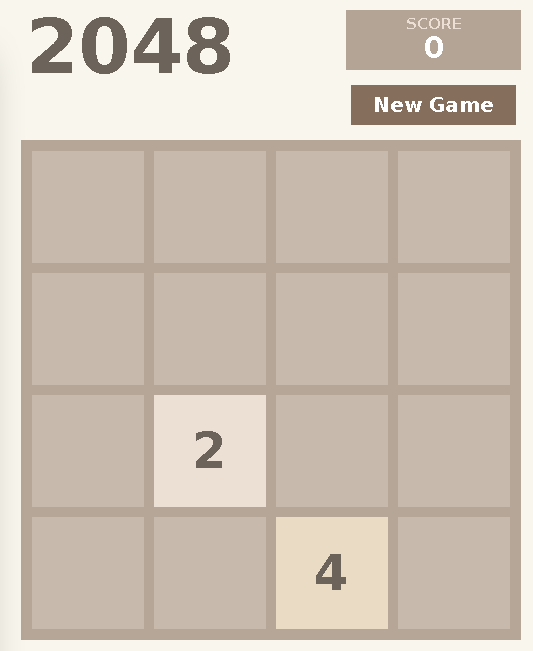
\includegraphics[width=0.3\textwidth]{mygame.png}
    \caption{Initial game state seen by the user.}
    \label{Figure 1:}
\end{figure}

\newpage

\section{Design Overview}
\hspace{\parindent}This design of the game applies a Model View Controller (MVC) design pattern  which lays out the foundation of my design. This design pattern was used to separate the computational components from the input/output components. The model part of the MVC design pattern was included in the
\verb|Model| class. The view portion of the MVC design patter was included in the \verb|GameGUI| class.
The controller part of the MVC design pattern was written in the \verb|Controller| class. The individual
portion of the MVC design pattern all have their own sets of responsibilities. The model, in my design, 
was in charge of encapsulating the system's data and all of the operations that my system will perform
on the data which includes the board and the tiles that make up the board. The model in my design was basically in charge of handling all of the game logic and data manipulation that must take place to create a functioning game. The view, in my design, used to display the data that was manipulated by the model through the use of a graphical user interface (GUI). The view is what the user will see as observed in Figure 1 but it does not provide the system with any logical operations for the game as that was abstracted in the model portion. Lastly, the controller, in my design, was the class that handled the input which was given by the user. Its task was take in the input from the user and convert that input an operation that must be done on the board and displayed to the user. Both the controller and the view portions of my MVC design pattern depends on the state of the model.\\
\hspace{\parindent}This is how the MVC design pattern was used in my design of the system: the model class inherits the \verb|BoardOps| which defines what methods are needed to make sure all logical operations function as intended. The model also uses the \verb|Board| and \verb|TileT| classes as data types to store the information that is to be manipulated by the model class. The model class also stores the state of the board and the tiles that are on it at any given time. The view module (\verb|GameGUI|) instantiates an instance of the model class and uses it to display the current state of the board to the user. Finally, the controller (\verb|Controller|) instantiates a instance of the view, takes in user input, and modifies that view for whatever the given input was.

\begin{figure}[h]
    \centering
    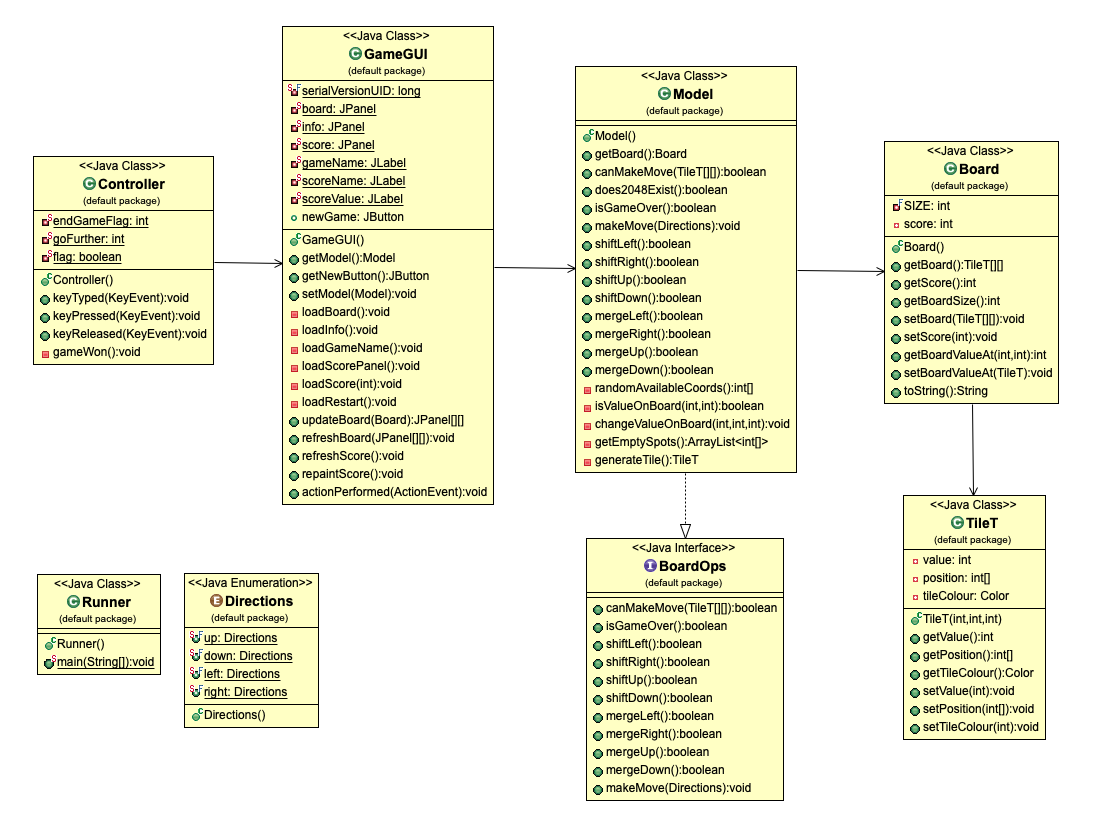
\includegraphics[width=0.8\textwidth]{A4uml.png}
    \caption{UML diagram for my game.}
    \label{Figure 2:}
\end{figure} 

\newpage

\section{Likely Changes}
\begin{itemize}
  \item One likely change that my design has taken into account is the ability for the board size to be dynamic (easily changed). I have designed for this change because in my \verb|Board| class I have a constant that represents the size of the board. This value can be easily changed to make the board smaller or larger based on the desire of the user. 
  \item Another likely change that my design has taken into account is the ability of incorporating more direction to be able to move in. I have accounted for this change by using an enumerated class for the movement directions of the board. Since the enumerated class abstracts the directions that the board can move in, it would be fairly straightforward to add functionality of various other directional moves, such as diagonal. 
  \item Also, a likely change that I have thought about with my design is the likely change of the required winning score (currently 2048). This can be easily changed in my controller class where I check if the winning tile has been created. It can be increased or decreased based on how difficult the game the user wants to play. 
  \item With my current design, I have also thought about a likely change that would change the way my program would get the user input to indicate a move in the game. As of my current design, I use the arrow keys on a keyboard, but this can easily be changed to any key on the keyboard that they user wishes to use.
  \item Finally, another likely change that I have accounted for with my current design of this system is that the winning/ending conditions can be modified. This can allow for various difficulties of the same game based on the user's desires.
\end{itemize}

\newpage

\section* {Directions Module}

\subsection*{Module}

Directions

\subsection* {Uses}

None

\subsection* {Syntax}

\subsubsection* {Exported Constants}

None

\subsubsection* {Exported Types}

Directions = \{\\
    up, \textit{\#Upwards move direction}\\
    down, \textit{\#Downwards move direction}\\
    left, \textit{\#Move to the left}\\
    right \textit{\#Move to the right}\\
\}

\subsubsection* {Exported Access Programs}

None

\subsection* {Semantics}

\subsubsection* {State Variables}

None

\subsubsection* {State Invariant}

None

\subsubsection* {Assumptions}

None

\subsubsection* {Considerations}

When implementing in Java, use enums.

\newpage

\section* {Tiles Module}

\subsection*{Template Module}

TileT

\subsection* {Uses}

Color

\subsection* {Syntax}

\subsubsection* {Exported Constants}

None

\subsubsection* {Exported Types}

TileT = ?

\subsubsection* {Exported Access Programs}

\begin{tabular}{| l | l | l | p{5cm} |}
\hline
\textbf{Routine name} & \textbf{In} & \textbf{Out} & \textbf{Exceptions}\\
\hline
new TileT & $\mathbb{Z}$, $\mathbb{Z}$, $\mathbb{Z}$ & TileT & ~\\
\hline
getValue & & $\mathbb{Z}$ & ~\\
\hline
getPosition & & seq of $\mathbb{Z}$ & ~\\
\hline
getTileColour & & Color & ~\\
\hline
setValue & $\mathbb{Z}$ & & IllegalArgumentException\\
\hline
setPosition & seq of $\mathbb{Z}$ & & IllegalArgumentException\\
\hline
setTileColour & $\mathbb{Z}$ & & IllegalArgumentException\\
\hline
\end{tabular}

\subsection* {Semantics}

\subsubsection* {State Variables}

$\mathit{value}: \mathbb{Z}$\\
$\mathit{position}: \text{set of $\mathbb{Z}$}$\\
$\mathit{tileColor}: Color$

\subsubsection* {State Invariant}

$value \ge 0 \land \vert position \vert = 2$

\subsubsection* {Assumptions}

It is assumed that the tile will be powers of 2 with the smallest possible number being a 2(a value of 0 represents empty tile and is allowed). It is also assumed that the colour for each tile will be set in the view (GUI) of the program. We can also assume that the position coordinates are greater than equal to 0 and less than the board size. The \verb|setTileColour| method will be run before \verb|getTileColour| can be used.

\subsubsection* {Access Routine Semantics}

\noindent new TileT($\mathit{val}, \mathit{x}, \mathit{y}$):
\begin{itemize}
\item transition: $\mathit{value}, \mathit{position} := \mathit{val}, \{x, y\}$
\item output: none
\item exception: none
\end{itemize}

\noindent getValue():
\begin{itemize}
\item output: $out := \mathit{value}$
\item exception: none
\end{itemize}

\noindent getPosition():
\begin{itemize}
\item output: $out := \mathit{position}$
\item exception: none
\end{itemize}

\noindent getTileColour():
\begin{itemize}
\item output: $out := \mathit{tileColour}$
\item exception: none
\end{itemize}

\noindent setValue(val):
\begin{itemize}
\item transition: $value := \mathit{val}$
\item exception: $exc := (val < 0 \Rightarrow IllegalArgumentException)$
\end{itemize}

\noindent setPosition(newCoords):
\begin{itemize}
\item transition: $position := \mathit{newCoords}$
\item exception: $exc := (\vert newCoords \vert \neq 2 \Rightarrow IllegalArgumentException)$
\end{itemize}

\noindent setTileColour(val):
\begin{itemize}
\item transition: $tileColour := ((val > 2048 \Rightarrow Color(0, 0, 0) \vert (val = 0 \Rightarrow Color(205, 193, 180) \vert (val = 2 \Rightarrow Color(238, 228, 218) \vert (val = 4 \Rightarrow Color(236, 224, 202) \vert (val = 8 \Rightarrow Color(242, 177, 121) \vert (val = 16 \Rightarrow Color(236, 141, 85) \vert (val = 32 \Rightarrow Color(247, 124, 95) \vert (val = 64 \Rightarrow Color(234, 90, 56) \vert (val = 128 \Rightarrow Color(244, 216, 107) \vert (val = 256 \Rightarrow Color(242, 208, 75) \vert (val = 512 \Rightarrow Color(228, 193, 42) \vert (val = 1024 \Rightarrow Color(227, 186, 19) \vert (val = 2048 \Rightarrow Color(236, 196, 2) \vert True \Rightarrow True)$
\item exception: $exc := (val < 0 \Rightarrow IllegalArgumentException)$
\end{itemize}

\newpage

\section* {Board Operations Interface Module}

\subsection*{Interface Module}

BoardOps

\subsection* {Uses}

TileT, Directions

\subsection* {Syntax}

\subsubsection* {Exported Constants}

None

\subsubsection* {Exported Types}

None 

\subsubsection* {Exported Access Programs}

\begin{tabular}{| l | l | l | p{6cm} |}
\hline
\textbf{Routine name} & \textbf{In} & \textbf{Out} & \textbf{Exceptions}\\
\hline
canMakeMove & seq of seq of TileT & $\mathbb{B}$ & \\
\hline
isGameOver & & $\mathbb{B}$ & \\
\hline
shiftLeft & & $\mathbb{B}$ & \\
\hline
shiftRight & & $\mathbb{B}$ & \\
\hline
shiftUp & & $\mathbb{B}$ & \\
\hline
mergeDown & & $\mathbb{B}$ & \\
\hline
mergeLeft & & $\mathbb{B}$ & \\
\hline
mergeRight & & $\mathbb{B}$ & \\
\hline
mergeUp & & $\mathbb{B}$ & \\
\hline
mergeDown & & $\mathbb{B}$ & \\
\hline
makeMove & dir: Directions &  & \\
\hline
  
\end{tabular}
    
\subsubsection* {Considerations}

The sequence of sequences of type \verb|TileT| represent all of the tiles that are on the board at any given time and in any state of the board.

\newpage

\section* {Board Module}

\subsection*{Template Module}

Board

\subsection* {Uses}

TileT

\subsection* {Syntax}

\subsubsection* {Exported Constants}

SIZE = 4  \#Used to define the number of rows and columns on the board

\subsubsection* {Exported Types}

Board = ?

\subsubsection* {Exported Access Programs}

\begin{tabular}{| l | l | l | p{5cm} |}
\hline
\textbf{Routine name} & \textbf{In} & \textbf{Out} & \textbf{Exceptions}\\
\hline
new Board & & & \\
\hline
getBoard & & seq of seq of TileT & \\
\hline
getScore & & $\mathbb{Z}$ & \\
\hline
getBoardSize & & $\mathbb{Z}$ & \\
\hline
getBoardValueAt & $\mathbb{Z}$, $\mathbb{Z}$ & $\mathbb{Z}$ & \\
\hline
setBoard & seq of seq of TileT & & \\
\hline
setScore & $\mathbb{Z}$ & & IllegalArgumentException\\
\hline
setBoardValueAt & TileT & & \\
\hline
\end{tabular}

\subsection* {Semantics}

\subsubsection* {State Variables}

$\mathit{board}$: seq of seq of TileT\\
$\mathit{score}: \mathbb{Z}$

\subsubsection* {State Invariant}

$score \ge 0$

\subsubsection* {Assumptions}

It is assumed that the board will be a square (i.e., the same number of rows as columns). It will also be assumed that the SIZE constant will be greater than 1 for a proper game to be made with possible moves. Finally, if a value is being accessed from the board, its input coordinates are assumed to have values greater than or equal to zero and less than the board size.

\subsubsection* {Access Routine Semantics}

\noindent new Board():
\begin{itemize}
\item transition: $\mathit{board}, \mathit{score} := (\forall i: \mathbb{N} \vert i \in [0...|board| - 1] \cdot ((\forall j: \mathbb{N} \vert j \in [0...|board| - 1]) \land board_ij = TileT(0, i, j))), 0$
\item output: none
\item exception: none
\end{itemize}

\noindent getBoard():
\begin{itemize}
\item output: $out := \mathit{board}$
\item exception: none
\end{itemize}

\noindent getScore():
\begin{itemize}
\item output: $out := \mathit{score}$
\item exception: none
\end{itemize}

\noindent getBoardSize():
\begin{itemize}
\item output: $out := \mathit{SIZE}$
\item exception: none
\end{itemize}

\noindent getBoardValueAt(x, y):
\begin{itemize}
\item output: $out := board_{xy}.getValue()$
\item exception: none
\end{itemize}

\noindent setBoard(currBoard):
\begin{itemize}
\item transition: $board := \mathit{currBoard}$
\item exception: none
\end{itemize}

\noindent setScore(currScore):
\begin{itemize}
\item transition: $score := \mathit{currScore}$
\item exception: $exc := (currScore < 0 \Rightarrow IllegalArgumentException)$
\end{itemize}

\noindent setBoardValueAt(tile):
\begin{itemize}
\item transition: $board_{(tile.getPosition()_0), (tile.getPosition()_1)} := tile.getValue()$
\item exception: none
\end{itemize}

\newpage

\section* {Model Module}

\subsection*{Template Module inherits BoardOps}

Model

\subsection* {Uses}

BoardOps, Board, TileT, Directions

\subsection* {Syntax}

\subsubsection* {Exported Constants}

None

\subsubsection* {Exported Types}

Model = ?

\subsubsection* {Exported Access Programs}

\begin{tabular}{| l | l | l | p{5cm} |}
  \hline
  \textbf{Routine name} & \textbf{In} & \textbf{Out} & \textbf{Exceptions}\\
  \hline
  new Model & & Model & \\
  \hline
  getBoard & & Board & \\
  \hline
  canMakeMove & seq of seq of TileT & $\mathbb{B}$ & \\
  \hline
  does2048Exist & & $\mathbb{B}$ & \\
  \hline
  isGameOver & & $\mathbb{B}$ & \\
  \hline
  makeMove & Directions & & \\
  \hline
  shiftLeft & & $\mathbb{B}$ & \\
  \hline
  shiftRight & & $\mathbb{B}$ & \\
  \hline
  shiftUp & & $\mathbb{B}$ & \\
  \hline
  shiftDown & & $\mathbb{B}$ & \\
  \hline
  mergeLeft & & $\mathbb{B}$ & \\
  \hline
  mergeRight & & $\mathbb{B}$ & \\
  \hline
  mergeUp & & $\mathbb{B}$ & \\
  \hline
  mergeDown & & $\mathbb{B}$ & \\
  \hline
  
\end{tabular}

\subsection* {Semantics}

\subsubsection* {State Variables}

$\mathit{board}$: $Board$

\subsubsection* {State Invariant}

None

\subsubsection* {Assumptions}

The constructor will internalize the board with two randomly generated tiles where one will be generated and placed onto the board before another tile is constructed and placed on the board. It is also assumed that a function to generate random numbers is also present.

\subsubsection* {Access Routine Semantics}

\noindent new Model():
\begin{itemize}
\item transition: \#$procedural$ $specification$\\
this.board = new Board;\\
TileT tile1 = generateTile();\\
this.board.setBoardValueAt(tile1);\\
TileT tile2 = generateTile();\\
this.board.setBoardValueAt();
\item output: none
\item exception: none
\end{itemize}

\noindent getBoard( ):
\begin{itemize}
\item output: $out := \mathit{board}$
\item exception: none
\end{itemize}

\noindent canMakeMove(b):
\begin{itemize}
\item output: $out := (\forall i,j : \mathbb{N} \vert i \in [0...|b| - 1] \land j \in [0...|b| - 1] \cdot ((board.getBoardValueAt(i, j) = 0 \Rightarrow True) \vert (isValueOnBoard(i - 1, j) \land board.getBoardValueAt(i, j) = board.getBoardValueAt(i - 1, j) \Rightarrow True) \vert (isValueOnBoard(i + 1, j) \land board.getBoardValueAt(i, j) = board.getBoardValueAt(i + 1, j) \Rightarrow True) \vert (isValueOnBoard(i, j - 1) \land board.getBoardValueAt(i, j) = board.getBoardValueAt(i, j - 1) \Rightarrow True) \vert (isValueOnBoard(i, j + 1) \land board.getBoardValueAt(i, j) = board.getBoardValueAt(i, j + 1) \Rightarrow True) \vert (True \Rightarrow False))$\\   \#There are only possible moves where there is a 0 (empty spot) on the board or if two adjacent tiles in any direction are the same (can be merged)
\item exception: none
\end{itemize}

\noindent does2048Exist():
\begin{itemize}
\item output: $out := (\forall i,j \vert i \in [0...|b| - 1] \land j \in [0...|b| - 1] \cdot (board.getBoard()_{i,j}.getValue() = 2048 \Rightarrow True) \vert (True \Rightarrow False))$
\item exception: none
\end{itemize}

\noindent isGameOver():
\begin{itemize}
\item out: $out := \lnot canMakeMove(board.getBoard())$
\item exception: none
\end{itemize}

\noindent makeMove(dir):
\begin{itemize}
\item transition: $\mathit{normInd} := (canMakeMove(board.getBoard()) \Rightarrow ((dir = Directions.up \Rightarrow shiftUp() \land mergeUp) \vert (dir = Directions.down \Rightarrow shiftDown() \land mergeDown) \vert (dir = Directions.right \Rightarrow shiftRight() \land mergeRight) \vert (dir = Directions.left \Rightarrow shiftLeft() \land mergeLeft) \vert (True \Rightarrow True)))$\\
\#Keep track if a shift or merge occurred and if either one happened then generate a tile and set its board value at the tile's specified coordinates
\item exception: none
\end{itemize}

\noindent shiftLeft():
\begin{itemize}
\item out: $out := (\forall i,x,j : \mathbb{N} \vert i \in [0...board.getBoardSize() - 1] \land x \in [0...|board.getBoard()_i| - 2] \land j \in [1...|board.getBoard()_i| - 1] \vert (board.getBoardValueAt(i, j - 1) = 0 \land \lnot (board.getBoardValueAt(i, j) = 0) \Rightarrow True) \vert (True \Rightarrow False)))$\\
\#Whenever we return True (meaning we can shift left), we must also perform the actual shifting of the tile. This can be done by changing the  value directly to its left to the value of the tile we are on currently and change the current spot on the board with a value of zero.
\item exception: none
\end{itemize}

\noindent shiftRight():
\begin{itemize}
\item out: $out := (\forall i,x,j : \mathbb{N} \vert i \in [0...board.getBoardSize() - 1] \land x \in [0...|board.getBoard()_i| - 2] \land j \in [1...|board.getBoard()_i| - 2] \vert (board.getBoardValueAt(i, j + 1) = 0 \land \lnot (board.getBoardValueAt(i, j) = 0) \Rightarrow True) \vert (True \Rightarrow False)))$\\
\#Whenever we return True (meaning we can shift right), we must also perform the actual shifting of the tile. This can be done by changing the  value directly to its right to the value of the tile we are on currently and change the current spot on the board with a value of zero.
\item exception: none
\end{itemize}

\noindent shiftUp():
\begin{itemize}
\item out: $out := (\forall j,x,i : \mathbb{N} \vert j \in [0...board.getBoardSize() - 1] \land x \in [0...|board.getBoard()_i| - 2] \land i \in [|board.getBoard()_i| - 2...1] \vert (board.getBoardValueAt(i - 1, j) = 0 \land \lnot (board.getBoardValueAt(i, j) = 0) \Rightarrow True) \vert (True \Rightarrow False)))$\\
\#Whenever we return True (meaning we can shift up), we must also perform the actual shifting of the tile. This can be done by changing the  value directly above it to the value of the tile we are on currently and change the current spot on the board with a value of zero.
\item exception: none
\end{itemize}

\noindent shiftDown():
\begin{itemize}
\item out: $out := (\forall j,x,i : \mathbb{N} \vert j \in [0...board.getBoardSize() - 1] \land x \in [0...|board.getBoard()_i| - 2] \land i \in [0...|board.getBoard()_i| - 2] \vert (board.getBoardValueAt(i + 1, j) = 0 \land \lnot (board.getBoardValueAt(i, j) = 0) \Rightarrow True) \vert (True \Rightarrow False)))$\\
\#Whenever we return True (meaning we can shift down), we must also perform the actual shifting of the tile. This can be done by changing the  value directly below it to the value of the tile we are on currently and change the current spot on the board with a value of zero.
\item exception: none
\end{itemize}

\noindent mergeLeft():
\begin{itemize}
\item out: $out := (\forall i,j : \mathbb{N} \vert i \in [0...board.getBoardSize() - 1] \land j \in [0...|board.getBoard()_i| - 1] \vert (\lnot (board.getBoardValueAt(i, j - 1) = 0) \land \lnot (board.getBoardValueAt(i, j) = 0) \Rightarrow (board.getBoardValueAt(i, j) = board.getBoardValueAt(i, j - 1)) \Rightarrow True) \vert (True \Rightarrow False)))$\\
\#Whenever we return True (meaning we can merge left), we must also perform the actual merging of the tiles. This is accomplished by combining the value of both the tiles into one (2x) and setting its location to the original adjacent left title of the two. We must also change the tile at (i, j) to zero, update the score, and perform a left shift.
\item exception: none
\end{itemize}

\noindent mergeRight():
\begin{itemize}
\item out: $out := (\forall i,j : \mathbb{N} \vert i \in [0...board.getBoardSize() - 1] \land j \in [0...|board.getBoard()_i| - 2] \vert (\lnot (board.getBoardValueAt(i, j) = 0) \land \lnot (board.getBoardValueAt(i, j + 1) = 0) \Rightarrow (board.getBoardValueAt(i, j) = board.getBoardValueAt(i, j + 1)) \Rightarrow True) \vert (True \Rightarrow False)))$\\
\#Whenever we return True (meaning we can merge right), we must also perform the actual merging of the tiles. This is accomplished by combining the value of both the tiles into one (2x) and setting its location to the original adjacent right title of the two. We must also change the tile at (i, j) to zero, update the score, and perform a right shift.
\item exception: none
\end{itemize}

\noindent mergeUp():
\begin{itemize}
\item out: $out := (\forall j,i : \mathbb{N} \vert j \in [0...board.getBoardSize() - 1] \land i \in [0...|board.getBoard()_i| - 2] \vert (\lnot (board.getBoardValueAt(i, j) = 0) \land \lnot (board.getBoardValueAt(i + 1, j) = 0) \Rightarrow (board.getBoardValueAt(i, j) = board.getBoardValueAt(i + 1, j)) \Rightarrow True) \vert (True \Rightarrow False)))$\\
\#Whenever we return True (meaning we can merge up), we must also perform the actual merging of the tiles. This is accomplished by combining the value of both the tiles into one (2x) and setting its location to the original adjacent up title of the two. We must also change the tile at (i, j) to zero, update the score, and perform a right shift.
\item exception: none
\end{itemize}

\noindent mergeDown():
\begin{itemize}
\item out: $out := (\forall j,i : \mathbb{N} \vert j \in [0...board.getBoardSize() - 1] \land i \in [0...|board.getBoard()_i| - 2] \vert (\lnot (board.getBoardValueAt(i, j) = 0) \land \lnot (board.getBoardValueAt(i - 1, j) = 0) \Rightarrow (board.getBoardValueAt(i, j) = board.getBoardValueAt(i - 1, j)) \Rightarrow True) \vert (True \Rightarrow False)))$\\
\#Whenever we return True (meaning we can merge down), we must also perform the actual merging of the tiles. This is accomplished by combining the value of both the tiles into one (2x) and setting its location to the original adjacent down title of the two. We must also change the tile at (i, j) to zero, update the score, and perform a down shift.
\item exception: none
\end{itemize}

\subsection*{Local Functions}

\noindent isValueOnBoard: $\mathbb{Z} \times \mathbb{Z}  \rightarrow \mathbb{B}$\\
\noindent
isValueOnBoard(x, y) $\equiv ((x \ge 0 \land x < board.getBoardSize() \land y \ge 0 \land y < board.getBoardSize()) \Rightarrow True \vert True \Rightarrow False)$
\textit{\#Returns whether or not a pair of integers representing the coordinates of the  board are actually in the bounds of the board.}
~\\

\noindent getEmptySpots: No Input  $\rightarrow$ seq of seq[2] of $\mathbb{Z}$\\
\noindent
getEmptySpots() $\equiv [i,j : \mathbb{N} \vert i \in [0...board.getBoardSize() - 1] \land j \in [0...board.getBoardSize() - 1] : (board.getValueAt(i, j) = 0 \Rightarrow \langle i,j \rangle)]$
\textit{\#Returns all of the locations (as a sequence of [2]) that are empty (value of 0) on the board.}
~\\

\noindent randomAvailableCoords: No Input  $\rightarrow$ seq[2] of $\mathbb{Z}$\\
\noindent
randomAvailableCoords() $\equiv getEmptySpots.get(random.nextInt(|getEmptySpots()|))$
\textit{\#Returns a random coordinate on the board from all of the available spots on the board. This function assumes that a random function that can chose a random integer is available to use.}
~\\

\noindent changeValueOnBoard: $\mathbb{Z} \times \mathbb{Z} \times \mathbb{Z}\rightarrow$ No Output\\
\noindent
changeValueOnBoard(val, x, y) $\equiv (isValueOnBoard(x, y) \Rightarrow (board.getBoard_{x,y}.setPosition(\langle x,y \rangle)) \land board.setBoardValueAt(TileT(val, x, y)))$\\
\textit{\#This method is used to change the value of a tile after a shift or merge move has been successfully executed only if there exists a possible tile location at the specified board coordinates.}
~\\

\noindent generateTile: No Input $\Rightarrow$ TileT\\
\noindent
generateTile() $\equiv (random.nextDouble() < 0.7 \Rightarrow TileT(2, coords[0], coords[1])) \vert (TileT(4, coords[0], coords[1]))$
\textit{\#This method generates a random tile (2 at the beginning and one every time we successfully shift or merge) at a random available location (variable coords here represents the coordinate generated by the randomAvailableCoords() method). It has a 70\% probability of generating a tile with a value of 2 and a 30\% probability of generating a tile with a value of 4. This function assumes that a random function is available to generate decimal values from 0 to 1.}
~\\

\newpage

\section* {GameGUI Module}

\subsection*{Template Module inherits ActionListener, JFrame}

GameGUI

\subsection* {Uses}

Model, Board, TileT, JLabel, JPanel, JButton, JFrame, ActionListener

\subsection* {Syntax}

\subsubsection* {Exported Constants}

serialVersionUID = 1L   \#This constant is enforced by JFrame

\subsubsection* {Exported Types}

GameGUI = ?

\subsubsection* {Exported Access Programs}

\begin{tabular}{| l | l | l | p{5cm} |}
\hline
\textbf{Routine name} & \textbf{In} & \textbf{Out} & \textbf{Exceptions}\\
\hline
new GameGUI & & GameGUI & ~\\
\hline
getModel & & Model & ~\\
\hline
getNewButton & & JButton & ~\\
\hline
setModel & Model & & ~\\
\hline
loadBoard & & & ~\\
\hline
loadInfo & & & ~\\
\hline
loadGameName & & & ~\\
\hline
loadScorePanel & & & ~\\
\hline
loadScore & & & ~\\
\hline
loadRestart & & & ~\\
\hline
updateBoard & Board & seq of seq of JPanel & ~\\
\hline
refreshBoard & seq of seq of JPanel & & ~\\
\hline
refreshScore & & & ~\\
\hline
repaintScore & & & ~\\
\hline
actionPerformed & ActionEvent & & ~\\
\hline
\end{tabular}

\subsection* {Semantics}

\subsubsection* {Environment Variables}
window: This uses a part of the computer screen to display the graphical user interface of the game and its related visual operations.

\subsubsection* {State Variables}

$\text{m}: \text{Model}$\\
$\text{board}$: \text{JPanel}\\
$\text{info}$: \text{JPanel}\\
$\text{score}$: \text{JPanel}\\
$\text{gameName}$: \text{JLabel}\\
$\text{scoreName}$: \text{JLabel}\\
$\text{scoreValue}$: \text{JLabel}\\
$\text{newGame}$: \text{JButton}

\subsubsection* {State Invariant}

None

\subsubsection* {Assumptions}

It is assumed that loading in a new game is not a part of the controller rather a GUI related functionality.

\subsubsection* {Access Routine Semantics}

\noindent new GameGUI():
\begin{itemize}
\item transition: window := The constructor will initialize the window size (550 by 700 pixels), allow the user to exit using the "x" button on the frame, and sets the background colour. Then it will set up the individual components that make up the game board such as the board itself, the score, the new game button, and the name of the game. It will use methods such as \verb|loadRestart|, \verb|loadBoard|, \verb|loadInfo|, \verb|loadGameName|, \verb|loadScorePanel|, \verb|loadScore|, and \verb|refreshBoard|. After all of the appropriate methods have been called, every component will be set visible to true so the user can see the game.
\item output: none
\item exception: none
\end{itemize}

\noindent getModel():
\begin{itemize}
\item output: $out := m$
\item exception: none
\end{itemize}

\noindent getNewButton():
\begin{itemize}
\item output: $out := newGame$
\item exception: none
\end{itemize}

\noindent setModel(model):
\begin{itemize} 
\item transition: $m := model$
\item exception: none
\end{itemize}

\noindent loadBoard():
\begin{itemize}
\item transition: window := Gives the board panel a grid layout based on the size of the board. Also gives the board some boarders in between the tiles on the board for visual purposes. THe background colour and the board's location are set. Then the board panel is added onto the main frame. 
\item exception: none
\end{itemize}

\noindent loadInfo():
\begin{itemize}
\item transition: window := This will initialize a panel to house the name of the game and all of the scoring information regarding the game. It will only set its location on the frame and its background colour.
\item exception: none
\end{itemize}

\noindent loadGameName():
\begin{itemize}
\item transition: window := This place the game name which is 2048 onto the information panel and set its font, background colour, and location on the panel.
\item exception: none
\end{itemize}

\noindent loadScorePanel():
\begin{itemize}
\item transition: window := This panel will house all of the scoring information regarding the game. After its background colour and location on the information panel have been set, it will be added onto the panel. Then the score label indicating to the user that the number they see is the score of the current game will be loaded onto the scoring panel with its colour, font, and location on the scoring panel set.
\item exception: none
\end{itemize}

\noindent loadScore():
\begin{itemize}
\item transition: window := This actual score value will be updated using this method. The score will be fetched from the model, converted to a string and placed into the label, all the visual effects will be taken care of, and its location on the scoring panel will be set. The score label will also be set so that the number will always be centered within the panel and then the label will be added to the scoring panel.
\item exception: none
\end{itemize}

\noindent loadRestart():
\begin{itemize}
\item transition: window := This will set up the new game button that will allow the user to start a new game without having to re-run the program. All of the button's visual aspects are set and its location on the frame is also set. The button will also have an action listener added to it so that it can respond to mouse clicks.  
\item exception: none
\end{itemize}

\noindent updateBoard(b):
\begin{itemize}
\item out: A 2D sequence of JPanels will be outputted that will help represent all of the tiles that are on the board. Iterate through all of the tiles on the board and set their tile colours. If the tile's value is not a zero then create a JPanel to represent the tile with its appropriate colour and place in the grid layout. A JLabel will be added to each tile panel for the value of the tile. If the value of the tile is a zero, then an empty tile will be constructed and placed onto the board at their specified locations. 
\item exception: none
\end{itemize}

\noindent refreshBoard(tiles):
\begin{itemize}
\item transition: window := This will first remove all of the tiles that are already on the board. It will then take the sequence of sequences of JPanels from the input to the function and add it to the board. This input will always come from the \verb|updateBoard| method.  
\item exception: none
\end{itemize}

\noindent refreshScore():
\begin{itemize}
\item transition: window := This will retrieve the current score from the current model (m) and use the \verb|loadScore| method to update the score on the game frame for the user to see.
\item exception: none
\end{itemize}

\noindent repaintScore():
\begin{itemize}
\item transition: window := This will will update the score visually by removing the score label off of the panel. Then it will call \verb|refreshScore| to update the current score and then this value will be repainted onto the frame.
\item exception: none
\end{itemize}

\noindent actionPerformed(e):
\begin{itemize}
\item transition: window := if $e.getSource()$ senses that the button was clicked, then it will recreate the entire game frame with the new game board and a reset score value.
\item exception: none
\end{itemize}

\newpage

\section* {Controller Module}

\subsection*{Template Module inherits KeyListener}

Controller

\subsection* {Uses}

GameGUI, KeyListener, Model, JOptionPane

\subsection* {Syntax}

\subsubsection* {Exported Constants}

None

\subsubsection* {Exported Types}

Controller = ?

\subsubsection* {Exported Access Programs}

\begin{tabular}{| l | l | l | p{5cm} |}
  \hline
  \textbf{Routine name} & \textbf{In} & \textbf{Out} & \textbf{Exceptions}\\
  \hline
  new Controller & & Controller & \\
  \hline
  keyPressed & KeyEvent & & ~\\
  \hline
  keyTyped & KeyEvent & & ~\\
  \hline
  keyReleased & KeyEvent & & ~\\
  \hline
  gameWon & & & ~\\
  \hline
  
\end{tabular}

\subsection* {Semantics}

\subsubsection* {State Variables}

$\text{game}: \text{GameGUI}$\\
$\text{endGameFlag}: \mathbb{Z}$\\
$\text{goFurther}: \mathbb{Z}$\\
$\text{flag}: \mathbb{B}$\\

\subsubsection* {State Invariant}

None

\subsubsection* {Assumptions}

It is assumed that the game will be played using the arrow keys and they will be mapped to the way the board moves.

\subsubsection* {Access Routine Semantics}

\noindent new Controller():
\begin{itemize}
\item transition: game := new GameGUI()\\
\#The constructor should also add a KeyListener to enable the game to respond to user input.
\item output: none
\item exception: none
\end{itemize}

\noindent keyPressed(e):
\begin{itemize}
\item transition: If the game is not over yet, this means that the user can still make moves. If the input is the up arrow keys, we will make a move using the right Direction enumeration and refresh the board accordingly. If the input is the down arrow keys, we will make a move using the down Direction enumeration and refresh the board accordingly. If the input is the right arrow keys, we will make a move using the right Direction enumeration and refresh the board accordingly. If the input is the left arrow keys, we will make a move using the left Direction enumeration and refresh the board accordingly. After a move has been made we will repaint the score and check if the game has been won (by checking if a 2048 tile exists on the board and if there is we will display an option for the user to quit or to continue with the game). Otherwise, we know the game has ended and upon the next move the user tries to make, they will be prompted that the game has ended and the game will close.
\item exception: none
\end{itemize}

\noindent keyPressed(e):
\begin{itemize}
\item transition: none
\item output: none
\item exception: none\\
\#This method is not used in the implementation of the game and is just there as part of the KeyListener interface.
\end{itemize}

\noindent keyReleased(e):
\begin{itemize}
\item transition: none 
\item output: none
\item exception: none\\
\#This method is not used in the implementation of the game and is just there as part of the KeyListener interface.
\end{itemize}

\noindent gameWon():
\begin{itemize}
\item transition: This method will only be used when the game has been won and it will display a window that will let the user know that they won and will ask them if they want to continue. If they select yes then the game will continue otherwise the game will end and the program will terminate.
\item exception: none
\end{itemize}

\newpage 

\section{My Answers to the Short Answer Questions}
\begin{enumerate}
  \item The UML diagram below shows the relationships between all of the classes in assignment 3.\\
  \begin{figure}[h]
    \centering
    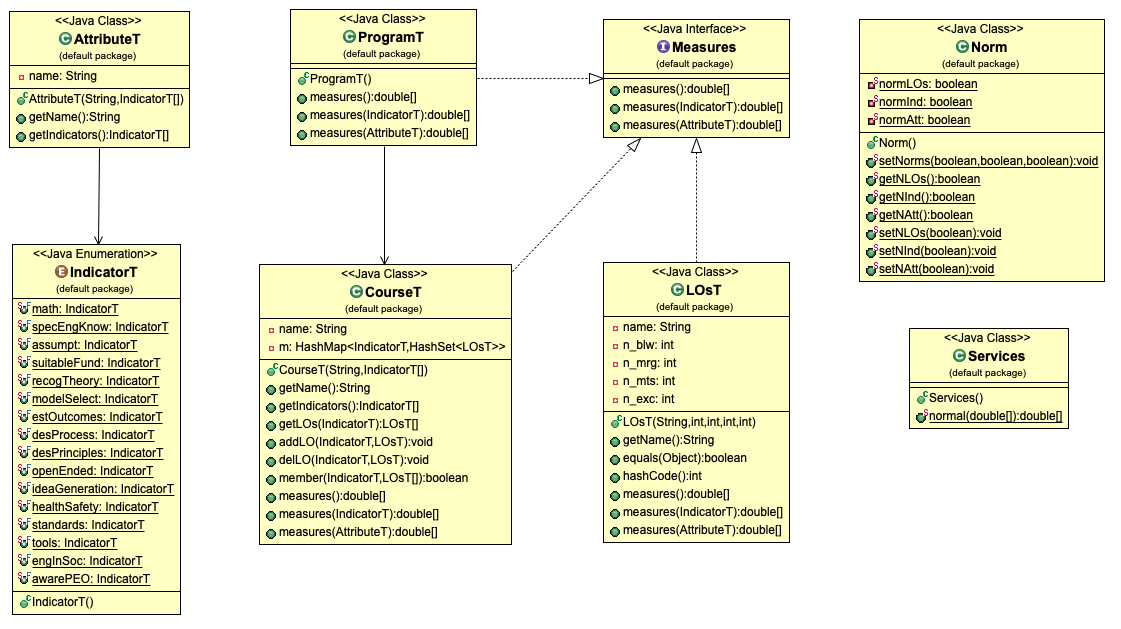
\includegraphics[width=1.0\textwidth]{A3uml.png}
    \caption{UML diagram for Assignment \#3.}
    \label{Figure 3:}
  \end{figure}
  \newpage
  \item Below is the control flow diagram of the convex hull algorithm.\\
  \begin{figure}[h]
    \centering
    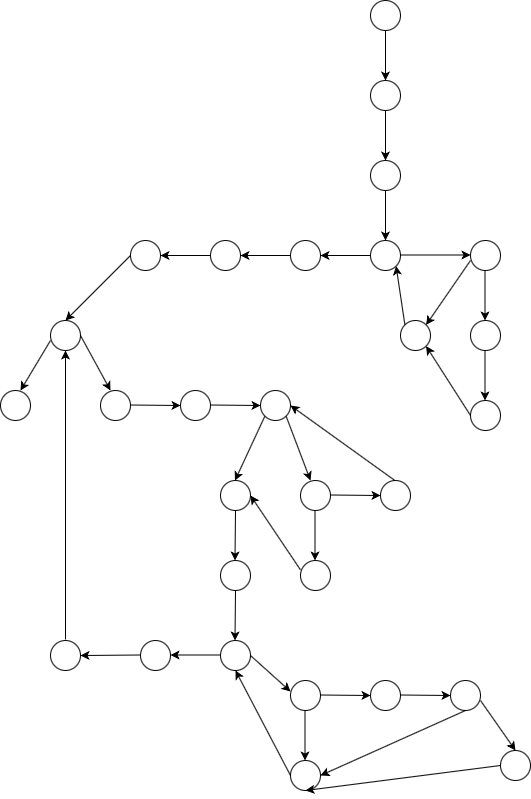
\includegraphics[width=0.5\textwidth]{controlflow.png}
    \caption{Convex Hull algorithm control flow diagram.}
    \label{Figure 4:}
  \end{figure}
\end{enumerate}

\newpage

\section{Design Critique}
\hspace{\parindent}Looking back at my design now, I can critique it in terms of consistency, essentiality, generality, minimality, cohesion, and information hiding. To begin with, my design is considered consistent. This is due to the fact that the naming conventions used, the ordering of parameters in argument lines, and the way that I decided to handle the exceptions I threw. My naming conventions were consistent because, for example, I always used x and y to denote the coordinates of a specific tile on the game board. I also believe that my specification and design was consistent because I always handled exceptions that were either related to the incorrect type or the passed in variables did not fit inside the domain of the inputs with a consistent type of exception that was being thrown (\verb|IllegalArgumentException|). Another reason why my design is deemed consistent is due to the fact that I followed a very specific naming convention for methods and variables throughout my specification (camel case). There was one place where I broke the consistency principle. This was where I had 2 methods that were named the same \verb|getBoard()| but from two different sources. Moving forward, my specification and design displays essentiality because all of my access routines are given one specific task to carry out. For the most part, my design was essential, but in my \verb|GameGUI| class, I had methods that were doing multiple things such as \verb|loadScorePanel| which was setting up multiple components of the panel at the same time, violating the principle of essentiality. My design, for the most part, was also quite general. This is due to the fact that including an interface for the board operations abstracts the necessary methods related to the operations of the board. I decided to do it this way because it makes the board operations more maintainable because if we wanted to add more operations in the future, we could add them to the interface and we would automatically know that we need to implement it in the  \verb|Model| class. Another reason why I made the board operations an interface was because it made it easier to understand and implement the MVC design pattern. This was due to the fact that it was easier to see what operations were vital to the operation of the game and it helped achieve the essentiality design principle. Moving onto minimality, my design and specification was, for the most part minimal, but there were a few places where I broke this design principle. There were a few places within the \verb|GameGUI| class where I had multiple transitions in one method as I discussed above. Also, I broke this principle in my \verb|Model| class because my shift and merge methods were doing more than one transition or output at once, which breaks this design principle. Other than that, my specification was minimal because every access routine in, for example, \verb|TileT| and \verb|Board| had either a single transition or output (only in charge of one specific operation). Speaking in terms of cohesion and couping, my design and specification achieves high cohesion and low coupling with the help of the MVC design pattern. This is due to the fact that the MVC design pattern demonstrates high cohesion as it groups all of the classes that accomplish related responsibilities together in either the model, view, or controller. The MVC design patter helps me achieve low coupling is due to the fact that since MVC groups classes with related functionalities together, they do not have any relationships with each other since they do not need each other's functionalities to function properly. Lastly, my specification and design achieves information hiding to a high degree. This is due to the fact that you cannot directly access any state variables outside from the class that they were defined in and you cannot change any of the state variable by directly accessing the variable itself outside the class. I showcase information hiding in my design by having accessors and mutators for all of my state variables (where applicable) so that I can change and/or access them outside the class that they were defined in. These are the strengths and weaknesses of my design and specification in terms of the design principles that we have studied. \\
\hspace{\parindent}To further critique my design, I would like to discuss some of the design decisions that I made while constructing this game. The first design decision that I would like to discuss is the fact that how I made my \verb|Model|, \verb|GameGUI|, and \verb|Controller| all abstract data types (ADTs). I decided to design my modules in such a way because I though that it would be easier to implement the functionality of creating a new game whenever the user feels like to restart the game. This really helped me out when I actually implemented the functionality because I simply had to call the model, view, and/or controller again to reset it whenever the user wanted a new game to be instantiated. Another design decision that I made was not to test my controller. This was due to the fact that all of the access routines that the controller was made up of was built using the methods that came from the view and/or the model. This meant that I only needed to test the \verb|Model| (in \verb|TestGame|). Another design decision that I made was naming 2 methods from different classes the same name. I did this so that I would understand what each one of them was doing easily and since both were doing the same job, I decided to name them the same so that I would avoid confusing myself. Even though the \verb|BoardOps| interface was not needed in my design, I decided to keep it in my design because it helped keep my operations organized and I would get a good indication if an operation was essential or not. The last design decision that I would like to talk about is my  decision to throw errors. If an error occurs, it would crash the program but it would also tell us that the program was supposed to crash as there was an unexpected input provided to the program that it did not know how to handle. Now I would like to shift my focus and talk about my testing methodologies. I designed my test cases in such a way so that all of my access routines from the classes that I was testing were tested at least once. This allowed my tests to explore and execute all possible paths in my program. Designing my test cases in such a way ensured that my tests would bring any errors or any unusual in my code to light before they impact other functionalities in my code. I also included test cases that raised the errors that I threw so that I can validate that the program operates correctly when it faces unknown inputs. Finally, when testing game moves in \verb|TestGame|, I decided to test making a move by verifying if all the tiles merged and shifted correctly and if a random tile was generated. I did not explicitly check if the random tile was generated because there is no way to know where it was generated due to the fact that the random functions were used to create the random generation of tiles, so I decided to check if a tile was different from a zero tile (empty tile) that was not included in a shift or merge. In conclusion, these are the design decision that I thought should be made to make the understandability and functionality of the game optimal and easy to understand from the user's perspective.

\end {document} 
